\documentclass{beamer}
\usepackage[T2A]{fontenc}
\usepackage[utf8]{inputenc}
\usepackage[english, russian]{babel}
\usepackage{graphicx, mathtools}
\graphicspath{{images/}}

\usetheme{Madrid}
\usecolortheme{default}

\title{О функции Миттаг-Леффлера и её приложениях в теории дифференциальных уравнений в дробных производных}
\date{25.06.2021}
\author{Тарасова Екатерина Сергеевна}

\setbeamertemplate{frametitle}[default][center]
\setbeamertemplate{navigation symbols}{}
\setbeamertemplate{footline}[page number]
\setbeamertemplate{caption}[numbered]

\DeclarePairedDelimiter{\norm}{\lVert}{\rVert}

\begin{document}

    \frame{\titlepage}

    \begin{frame}
        \frametitle{Постановка задачи}
        В данной работе ставятся и решаются следующие задачи:
        \begin{enumerate}
            \item 1;
            \item 2;
            \item 3.
        \end{enumerate}
    \end{frame}

    \begin{frame}
        \frametitle{Функция априорной оценки}
        Функция априорной оценки $\mathcal{C}$ на интервале $[0, T]$:
        \begin{equation}
            \label{eq:C}
            \norm{x(t)}^2 \leq E_q(t)\norm{x_0} + \int_0^t (t-s)^{q-1} E_{q,q}((-d+a)(t-s)^q)G(s)ds
        \end{equation}
        где
        \begin{equation*}
            \begin{aligned}
                &E_{\alpha, \beta}(z) = \sum_{k=0}^\infty \frac{z^k}{\Gamma (\alpha k + \beta)} - \text{функция Миттаг-Леффлера,}\\
                &\Gamma(z) = \int_0^{+\infty} t^{z-1} e^{-t} dt, \quad z \in \mathbb{C}, \quad Re(z) > 0 - \text{Гамма-функция Эйлера.}
            \end{aligned}
        \end{equation*}
    \end{frame}

    \begin{frame}
        \frametitle{График функции априорной оценки}
        \begin{figure}
            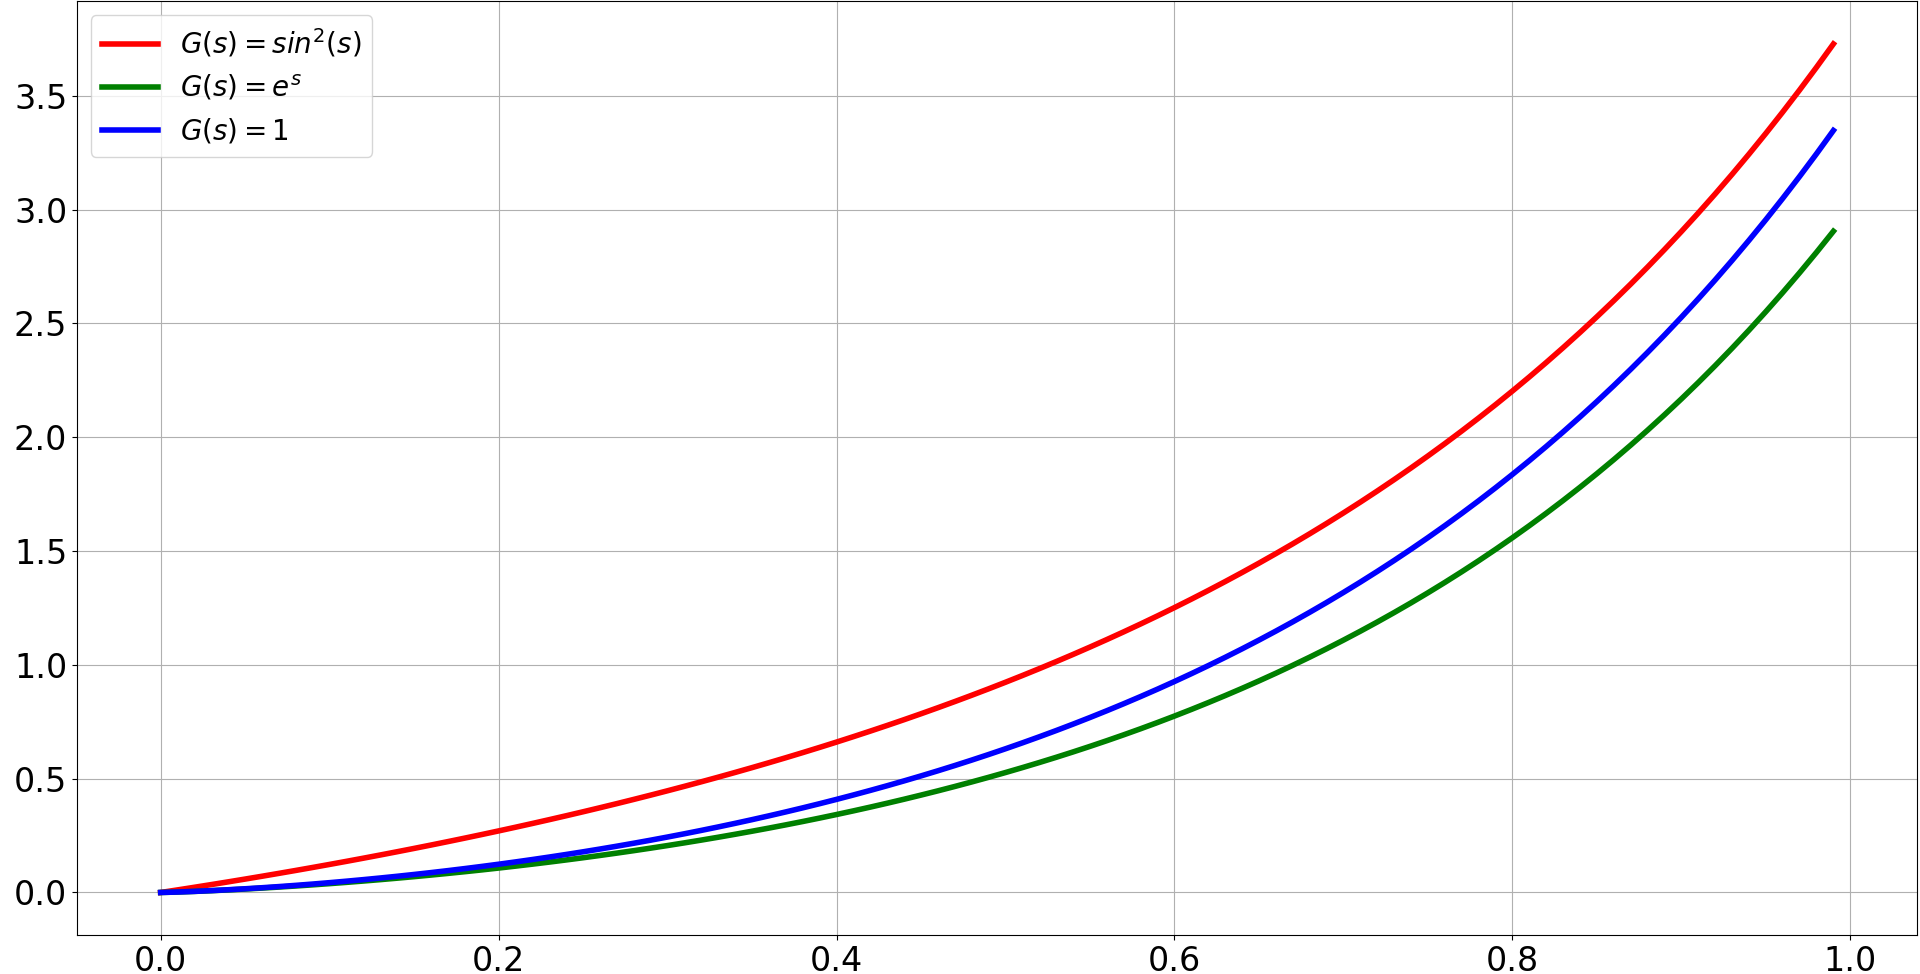
\includegraphics[width=0.75\linewidth]{plot}
            \caption{График функции (\ref{eq:C}) при $x_0 = 1$; $q = 0.5$; $d = 2$; $a = 1$; $t = 1$.}
        \end{figure}
    \end{frame}

    \begin{frame}
        \begin{block}{}
            \centerline{\color{blue}Спасибо за внимание!}
        \end{block}
    \end{frame}

\end{document}